\section{Task 2}

\begin{figure}[H]
\centering
\begin{circuitikz}[american voltages]

    % Nodes
    \node[circle, draw=black, fill=none, thick, inner sep=2pt] (VinTop) at (-4,1.5) {};
    \node[circle, draw=black, fill=none, thick, inner sep=2pt] (VinBot) at (-4,-1.5) {};

    \node[circle, fill=black, inner sep=0pt] (N1) at (-0.3,1.5) {};
    \node[circle, fill=black, inner sep=0pt] (N2) at (-0.3,-1.5) {};
    \node[circle, fill=black, inner sep=0pt] (Top) at (1.5,1.5) {};
    \node[circle, fill=black, inner sep=0pt] (Bot) at (1.5,-1.5) {};

    \node[circle, draw=black, fill=none, thick, inner sep=2pt] (VoutTop) at (3.5,1.5) {};
    \node[circle, draw=black, fill=none, thick, inner sep=2pt] (VoutBot) at (3.5,-1.5) {};

    % Input voltage
    \draw (VinTop) to[open, v^=$U_i$] (VinBot);

    % Bottom rail
    \draw (VinBot) -- (Bot) -- (VoutBot);

    % Top path with resistor
    \draw (VinTop) to[R=$2\,\mathrm{k}\Omega$, i>^=$I_R$] (N1) -- (Top) -- (VoutTop);

    % Parallel branches
    \draw (N1) to[D, l=Si] (N2);                 % diode branch
    \draw (Top) to[R=$5\,\mathrm{k}\Omega$] (Bot); % resistor branch

    % Output voltage
    \draw (VoutTop) to[open, v^=$U_0$] (VoutBot);

\end{circuitikz}
\caption{Diode and resistor in parallel between output nodes.}
\label{fig:parallel_diode_resistor}
\end{figure}

\noindent
Before $U_0$ reach $0.7V$ all current pass through the $5k\Omega$ resistor. We then have this:
\[
I_R = \frac{U_i}{2k+5k} \quad U_0 = U_i - 2\left(\frac{U_i}{7k}\right)
\]

\noindent
By checking when $U_0$ equals 0.7 we solve for $U_i$ and get $U_i = 0.98V$. This means that when input voltage is greater than $0.98V$ we have output voltage of $0.7V$ constantly. When input is negative, the current is reversed and the diode shuts off, and in that case we can calculate output as.

\[
U_0 = 5k \cdot \left(\frac{U_i}{2k + 5k}\right) \rightarrow U_0 = U_i \cdot \frac{5}{7}
\]

\noindent
When the diode activates, the current will have a maximum of $9.3V$ going over the $2k$ resistor. When the diode is shut off, the current will be decided by voltage over resistor. The highest and lowest possible values are as below.

\[
I_{R\uparrow} = \frac{9.3V}{2k\Omega} = 4.65mA
\]
\[
U_{0\downarrow} = -10V \cdot \frac{5k\Omega}{2k\Omega + 5k\Omega} = -7.14V
\]
\[
I_{R\downarrow} = \frac{-7.14V}{5k\Omega} = -1.42mA
\]

\noindent
The graphs are shown below.

\begin{figure}[H]
\centering
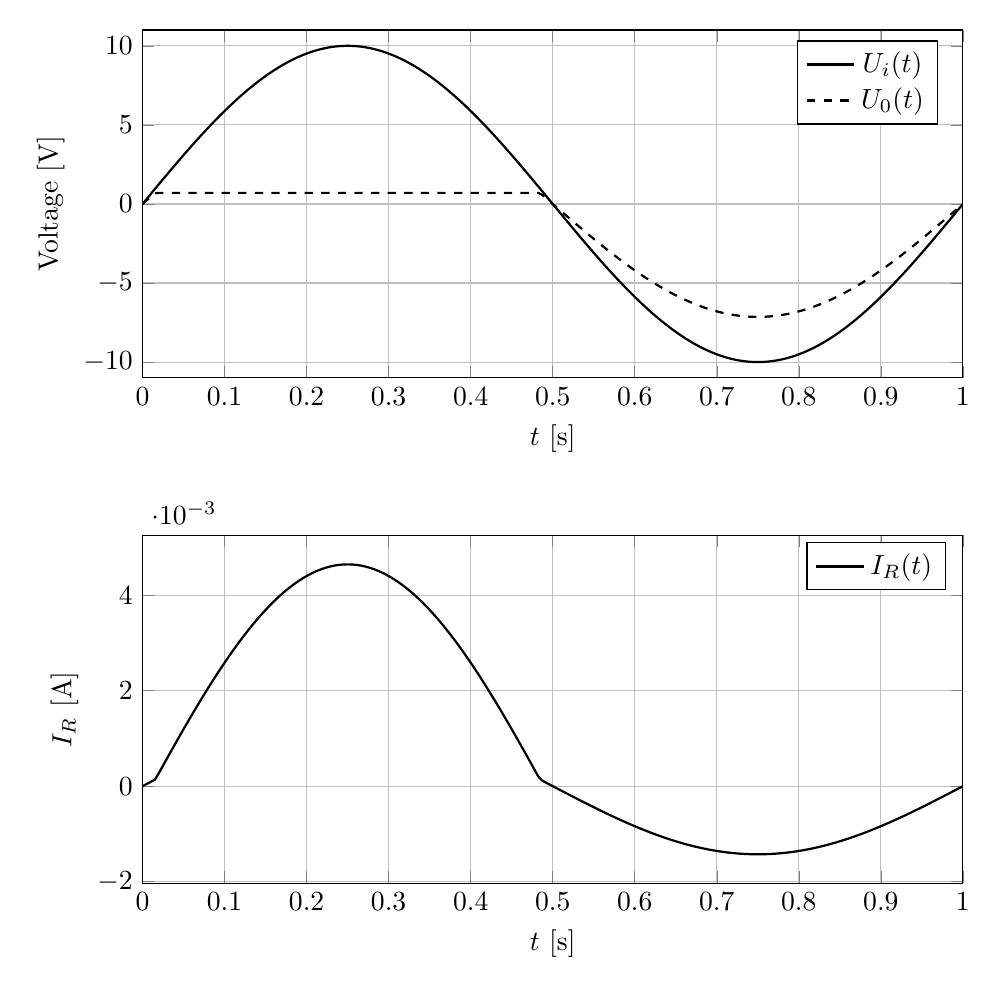
\begin{tikzpicture}

% ---- Voltage plot ----
\begin{axis}[
    width=12cm,
    height=6cm,
    xlabel={$t$ [s]},
    ylabel={Voltage [V]},
    xmin=0, xmax=1,
    ymin=-11, ymax=11,
    grid=both,
    legend pos=north east,
    domain=0:1,
    samples=200
]

\addplot[thick]
{10*sin(deg(2*pi*x))};
\addlegendentry{$U_i(t)$}

\addplot[thick, dashed]
{ (10*sin(deg(2*pi*x)) > 0.98) ? 0.7 : (5/7)*(10*sin(deg(2*pi*x))) };
\addlegendentry{$U_0(t)$}

\end{axis}

% ---- Current plot ----
\begin{axis}[
    at={(0,-2cm)},
    anchor=north west,
    width=12cm,
    height=6cm,
    xlabel={$t$ [s]},
    ylabel={$I_R$ [A]},
    xmin=0, xmax=1,
    grid=both,
    domain=0:1,
    samples=200
]

\addplot[thick]
{
(10*sin(deg(2*pi*x)) > 0.98)
? (10*sin(deg(2*pi*x)) - 0.7)/2000
: (10*sin(deg(2*pi*x)))/7000
};

\addlegendentry{$I_R(t)$}

\end{axis}

\end{tikzpicture}
\caption{Voltage and current in the diode circuit.}
\label{fig:diode_voltage_current}
\end{figure}